% SC4242 --- Chapter 4: Semantic Analysis & Type Systems (0->100 ground-up)
\chapter{Semantic Analysis and Type Systems}
\label{ch:semantic}

\begin{quote}
\emph{``Syntax asks `can I write this?' Semantics asks `what does it mean -- and is it allowed?'.''} --- Scopes, bindings, and types catch bugs before any code runs.
\end{quote}

\noindent\fbox{\parbox{\dimexpr\linewidth-2\fboxsep-2\fboxrule}{%
\textbf{From zero: we build here, no type theory assumed.} We define names, scopes, bindings, and types from sets and functions. Judgements, inference rules, and unification are introduced via pictures then formalism. No prior logic course is assumed.}}
\vspace{0.4em}

\section*{Learning Outcomes}
After this chapter you will be able to:
\begin{enumerate}[label=(L\arabic*)]
    \item distinguish lexical vs.\ dynamic scope and implement a scoped symbol table;
    \item resolve names, detect shadowing, and report precise ``undeclared identifier'' diagnostics;
    \item read and write typing judgements $\Gamma\vdash e:\tau$ and derivation trees;
    \item implement Hindley--Milner inference $\mathcal{W}$ with unification and let-generalisation;
    \item design coercions, overloading resolution, and gradual typing checks.
\end{enumerate}

% ============================================================
\section{Names, Scopes, and Bindings}
\label{sec:names}
\emph{Intuition:} a name is a use; a declaration is its binder. Scope is the region where that binder is visible. Like nested boxes---inner box shadows outer.

\begin{definition}[Scope and binding]
A \emph{declaration} binds identifier $x$ to an entity (variable, function, type). A \emph{use} is an occurrence of $x$. The \emph{scope} of a declaration is the set of program points where uses resolve to it. \emph{Lexical} (static) scope = nesting of blocks; \emph{dynamic} scope = most recent call on stack (rare, error-prone). NTU languages use lexical scope.
\end{definition}

\begin{example}[Shadowing]
\begin{lstlisting}[language=C]
int x = 1;          // outer x
{ int x = 2;        // inner x shadows
  print(x);         // 2
}
print(x);           // 1
\end{lstlisting}
Two distinct entities share spelling \texttt{x}; resolution picks the innermost enclosing binding. A symbol table must model this.
\end{example}

\paragraph{Symbol table as a stack of maps.} Enter scope $\to$ push new map; declare $x$ $\to$ insert in top map (error if already there---redeclaration); lookup $x$ $\to$ walk stack top-to-bottom; exit scope $\to$ pop. For efficient walking, chain entries via ``next in scope'' or hash with scope id. Fig.~\ref{fig:scope-tree} shows tree vs.\ stack view.

% TikZ 1: scope tree + symbol table stack
\begin{figure}[h]
\centering
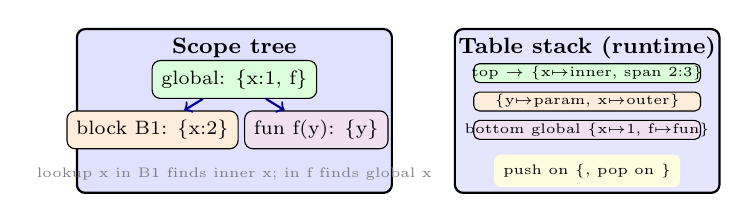
\begin{tikzpicture}[scale=0.80,every node/.style={font=\scriptsize}]
% scope tree
\draw[thick,fill=blue!12,rounded corners=3pt] (0,0) rectangle (5.0,2.6);
\node[font=\footnotesize\bfseries] at (2.5,2.3) {Scope tree};
\node[draw,fill=green!14,rounded corners=3pt] (g0) at (2.5,1.8) {global: \{x:1, f\}};
\node[draw,fill=orange!14,rounded corners=3pt] (g1) at (1.2,1.0) {block B1: \{x:2\}};
\node[draw,fill=violet!12,rounded corners=3pt] (g2) at (3.8,1.0) {fun f(y): \{y\}};
\draw[->,thick,blue!60!black] (g0)--(g1);
\draw[->,thick,blue!60!black] (g0)--(g2);
\node[font=\tiny,gray] at (2.5,0.3) {lookup x in B1 finds inner x; in f finds global x};
% stack view
\begin{scope}[xshift=6.0cm]
\draw[thick,fill=blue!10,rounded corners=3pt] (0,0) rectangle (4.2,2.6);
\node[font=\footnotesize\bfseries] at (2.1,2.3) {Table stack (runtime)};
\draw[fill=green!14,draw,rounded corners=2pt] (0.3,1.75) rectangle (3.9,2.05);
\node[font=\tiny] at (2.1,1.90) {top $\to$ \{x$\mapsto$inner, span 2:3\}};
\draw[fill=orange!14,draw,rounded corners=2pt] (0.3,1.30) rectangle (3.9,1.60);
\node[font=\tiny] at (2.1,1.45) {\{y$\mapsto$param, x$\mapsto$outer\}};
\draw[fill=violet!12,draw,rounded corners=2pt] (0.3,0.85) rectangle (3.9,1.15);
\node[font=\tiny] at (2.1,1.00) {bottom global \{x$\mapsto$1, f$\mapsto$fun\}};
\node[font=\tiny,fill=yellow!12,rounded corners=2pt] at (2.1,0.35) {push on \texttt{\{}, pop on \texttt{\}}};
\end{scope}
\end{tikzpicture}
\caption{Scopes as nested boxes: tree view (declaration sites) and stack view (table push/pop while walking the AST). Shadowing is stack shadowing.}
\label{fig:scope-tree}
\end{figure}

\begin{lstlisting}[language=Python]
class SymTab:
    def __init__(self): self.stack = [{}]          # global scope
    def enter(self): self.stack.append({})
    def exit(self): self.stack.pop()
    def declare(self, name, info):
        if name in self.stack[-1]: raise Redeclare(name)
        self.stack[-1][name] = info
    def lookup(self, name):
        for scope in reversed(self.stack):
            if name in scope: return scope[name]
        raise Undeclared(name)
    # visitor: walk AST, enter/exit at block/let/fun nodes
\end{lstlisting}

% ============================================================
\section{Type Systems: Judgements and Rules}
\label{sec:types}
\emph{Intuition:} types are lightweight specifications: ``this expression will produce an \texttt{int}''. A type system proves (at compile time) that no execution will confuse \texttt{int} with \texttt{string}.

\begin{definition}[Types and judgements]
Base types: \texttt{int}, \texttt{bool}, \texttt{string}. Compound: $\tau_1\to\tau_2$ (function), $\tau_1\times\tau_2$ (pair), $[\tau]$ (list), $\forall\alpha.\tau$ (polymorphic). \emph{Typing environment} $\Gamma$ is a map $x_1:\tau_1,\dots,x_n:\tau_n$. Judgement $\Gamma\vdash e:\tau$ reads ``under $\Gamma$, expression $e$ has type $\tau$''.
\end{definition}

Inference rules are fractions: premises above, conclusion below.
\begin{center}
\begin{tabular}{c}
\textsc{T-Var} $\displaystyle\frac{x:\tau\in\Gamma}{\Gamma\vdash x:\tau}$\quad
\textsc{T-Add} $\displaystyle\frac{\Gamma\vdash e_1:\texttt{int}\quad\Gamma\vdash e_2:\texttt{int}}{\Gamma\vdash e_1+e_2:\texttt{int}}$\\[1.2em]
\textsc{T-If} $\displaystyle\frac{\Gamma\vdash c:\texttt{bool}\quad\Gamma\vdash e_1:\tau\quad\Gamma\vdash e_2:\tau}{\Gamma\vdash \texttt{if }c\texttt{ then }e_1\texttt{ else }e_2:\tau}$\quad
\textsc{T-Abs} $\displaystyle\frac{\Gamma,x:\tau_1\vdash e:\tau_2}{\Gamma\vdash \lambda x.e:\tau_1\to\tau_2}$
\end{tabular}
\end{center}
A \emph{derivation tree} composes rules; its root is the program's type. If no derivation exists, the program is ill-typed.

% TikZ 2: typing derivation tree
\begin{figure}[h]
\centering
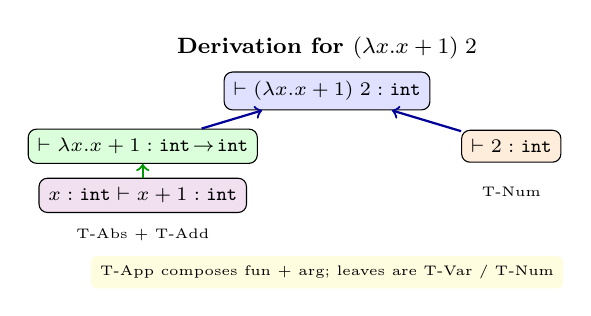
\begin{tikzpicture}[scale=0.78,every node/.style={font=\scriptsize}]
\node[font=\footnotesize\bfseries] at (5.0,2.7) {Derivation for $(\lambda x.x+1)\;2$};
% tree
\node[draw,fill=blue!12,rounded corners=3pt] (r) at (5.0,2.0) {$\vdash (\lambda x.x+1)\;2 : \texttt{int}$};
\node[draw,fill=green!14,rounded corners=3pt] (l) at (2.0,1.1) {$\vdash \lambda x.x+1 : \texttt{int}\!\to\!\texttt{int}$};
\node[draw,fill=orange!14,rounded corners=3pt] (a) at (8.0,1.1) {$\vdash 2:\texttt{int}$};
\node[draw,fill=violet!12,rounded corners=3pt] (b) at (2.0,0.3) {$x:\texttt{int}\vdash x+1:\texttt{int}$};
\node[font=\tiny] at (2.0,-0.35) {T-Abs + T-Add};
\node[font=\tiny] at (8.0,0.35) {T-Num};
\draw[->,thick,blue!60!black] (l)--(r);
\draw[->,thick,blue!60!black] (a)--(r);
\draw[->,thick,green!60!black] (b)--(l);
\node[font=\tiny,fill=yellow!12,rounded corners=2pt] at (5.0,-0.95) {T-App composes fun + arg; leaves are T-Var / T-Num};
\end{tikzpicture}
\caption{A typing derivation tree: each node is a judgement justified by an inference rule; composition mirrors the AST shape.}
\label{fig:typing-deriv}
\end{figure}

\begin{example}[Ill-typed and why]
\texttt{if 3 then 1 else 0} fails: premise $\Gamma\vdash 3:\texttt{bool}$ does not hold (\texttt{3} has \texttt{int}). Compiler error: ``expected \texttt{bool}, got \texttt{int} in condition''. Good errors quote the rule that failed and point at the offending subexpression's span.
\end{example}

% ============================================================
\section{Hindley--Milner Inference and Unification}
\label{sec:hm}
Monorphic checks need annotations; polymorphic inference invents them. \emph{Let-polymorphism}: \texttt{let id = \textbackslash x.x in id 3} gives \texttt{id} type $\forall\alpha.\alpha\to\alpha$, instantiated differently per use.

\begin{definition}[Unification]
Given equations $\tau_1=\sigma_1,\dots$, a \emph{unifier} is a substitution $S$ on type variables with $S(\tau_i)=S(\sigma_i)$. The \emph{most general unifier} (mgu) is the least committing; Robinson's algorithm finds it by structural recursion, with \emph{occurs check} $\alpha\notin\text{FV}(\tau)$ to reject $\alpha=\alpha\to\alpha$.
\end{definition}

Algorithm $\mathcal{W}(\Gamma,e)$ returns $(S,\tau)$ (substitution + type):
\begin{enumerate}[label=\arabic*.]
\item $e=x$: lookup $x:\forall\bar\alpha.\tau$ in $\Gamma$, freshen $\bar\alpha$ to new vars, return $(\emptyset,\tau')$.
\item $e=e_1\,e_2$: infer $(S_1,\tau_1)$ for $e_1$, $(S_2,\tau_2)$ for $S_1(e_2)$, fresh $\beta$, unify $S_2(\tau_1)=\tau_2\to\beta$, return.
\item $e=\lambda x.e_1$: fresh $\beta$ for $x$, infer $\Gamma,x:\beta\vdash e_1$, return $\beta\to\tau_1$.
\item $e=\texttt{let }x=e_1\texttt{ in }e_2$: infer $(S_1,\tau_1)$ for $e_1$, generalise free vars not in $S_1(\Gamma)$ to $\forall$, infer $e_2$ under extended $\Gamma$, compose.
\end{enumerate}

% TikZ 3: unification steps + generalisation
\begin{figure}[h]
\centering
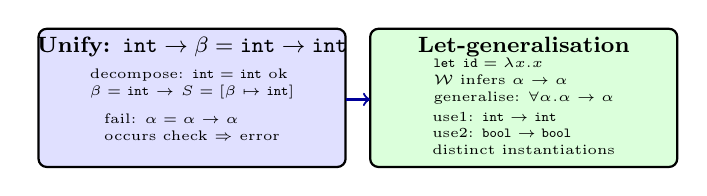
\begin{tikzpicture}[scale=0.78,every node/.style={font=\scriptsize}]
\draw[thick,fill=blue!12,rounded corners=3pt] (0,0) rectangle (5.0,2.25);
\node[font=\footnotesize\bfseries] at (2.5,1.95) {Unify: $\texttt{int}\to\beta = \texttt{int}\to\texttt{int}$};
\node[font=\tiny,align=left] at (2.5,1.35) {decompose: $\texttt{int}=\texttt{int}$ ok\\ $\beta = \texttt{int}$ $\to$ $S=[\beta\mapsto\texttt{int}]$};
\node[font=\tiny,align=left] at (2.5,0.65) {fail: $\alpha = \alpha\to\alpha$\\ occurs check $\Rightarrow$ error};
\draw[thick,fill=green!14,rounded corners=3pt] (5.4,0) rectangle (10.4,2.25);
\node[font=\footnotesize\bfseries] at (7.9,1.95) {Let-generalisation};
\node[font=\tiny,align=left] at (7.9,1.4) {$\texttt{let id}=\lambda x.x$\\ $\mathcal{W}$ infers $\alpha\to\alpha$\\ generalise: $\forall\alpha.\alpha\to\alpha$};
\node[font=\tiny,align=left] at (7.9,0.55) {use1: $\texttt{int}\to\texttt{int}$\\ use2: $\texttt{bool}\to\texttt{bool}$\\ distinct instantiations};
\draw[->,thick,blue!60!black] (5.0,1.1)--(5.4,1.1);
\end{tikzpicture}
\caption{Left: unification $\beta=\texttt{int}$ succeeds, recursive occurs-check fails. Right: let-generalisation gives polymorphism; each use freshens $\forall$-vars.}
\label{fig:unify-let}
\end{figure}

\begin{lstlisting}[language=Python]
def unify(t1, t2, subst):          # t = ('var',a) | ('con','int') | ('arr',l,r)
    t1, t2 = apply(subst,t1), apply(subst,t2)
    if t1 == t2: return subst
    if is_var(t1):
        if occurs(t1[1], t2): raise TypeError("occurs check")
        return compose({t1[1]: t2}, subst)
    if is_var(t2): return unify(t2, t1, subst)
    if t1[0]=='arr' and t2[0]=='arr':
        s = unify(t1[1], t2[1], subst)
        return unify(apply(s,t1[2]), apply(s,t2[2]), s)
    raise TypeError(f"cannot unify {t1} vs {t2}")
\end{lstlisting}

\paragraph{Coercions and overloading.} Languages insert implicit coercions (\texttt{int} $\to$ \texttt{float}) via elaboration; overloading resolves $+$ to integer-add vs.\ float-add vs.\ string-concat by type of operands (or type classes). Gradual typing adds \texttt{?} (unknown) with runtime checks at boundaries.

% ============================================================
\section{Chapter Notes}
Symbol tables date to assemblers; scoped tables are due to Dijkstra (block structure). Hindley--Milner (1969/78) underlies ML, Haskell, and Rust's trait inference. Damas--Milner $\mathcal{W}$ is linear in practice; production compilers memoise and parallelise. Pierce's \emph{Types and Programming Languages} is the rigorous reference; Appel Ch.~5 maps it to compiler implementation.

% ============================================================
\section{Exercises}
\label{sec:ch04-exercises}
\begin{enumerate}[label=E4.\arabic*, leftmargin=*, itemsep=0.8em]
\item \textbf{Scope implementation.} Extend \texttt{SymTab} to support (a) function scopes where params are in function's scope not caller's, and (b) \texttt{let x= e1 in e2} where \texttt{x} not visible in \texttt{e1}. Give visitor pseudocode and a test with shadowing depth 3.
\item \textbf{Derivation tree.} Derive $\vdash \texttt{let }f=\lambda x.x\texttt{ in }(f\;3,\;f\;\texttt{true}) : \texttt{int}\times\texttt{bool}$ using T-Let, T-Abs, T-App. Mark where generalisation happens.
\item \textbf{Unification trace.} Unify $(\alpha\to\alpha)\to\beta = (\texttt{int}\to\texttt{int})\to\texttt{bool}$ stepwise; show substitution composition. Then show $\alpha\to\beta = \beta\to\alpha$ yields $[\beta\mapsto\alpha]$ or $[\alpha\mapsto\beta]$---why many mgus?
\item \textbf{Occurs check.} Explain why $\mathcal{W}$ must reject $\lambda x.x\;x$ (self-application). Attempt to infer its type and pinpoint the equation $\alpha=\alpha\to\beta$ triggering occurs check.
\item \textbf{Coercion elaboration.} Design insertion for \texttt{int} $\le$ \texttt{float} with rule \texttt{int}+\texttt{float}$\to$\texttt{float} (coerce left). Elaborate \texttt{(1 + 2.0) + 3} to explicit \texttt{toFloat} calls and give typing derivation; where would a coercion lattice place \texttt{int}<:\texttt{float}?
\end{enumerate}
% End of Chapter 4
